\documentclass[]{article}
\usepackage{lmodern}
\usepackage{amssymb,amsmath}
\usepackage{ifxetex,ifluatex}
\usepackage{fixltx2e} % provides \textsubscript
\ifnum 0\ifxetex 1\fi\ifluatex 1\fi=0 % if pdftex
  \usepackage[T1]{fontenc}
  \usepackage[utf8]{inputenc}
\else % if luatex or xelatex
  \ifxetex
    \usepackage{mathspec}
  \else
    \usepackage{fontspec}
  \fi
  \defaultfontfeatures{Ligatures=TeX,Scale=MatchLowercase}
\fi
% use upquote if available, for straight quotes in verbatim environments
\IfFileExists{upquote.sty}{\usepackage{upquote}}{}
% use microtype if available
\IfFileExists{microtype.sty}{%
\usepackage{microtype}
\UseMicrotypeSet[protrusion]{basicmath} % disable protrusion for tt fonts
}{}
\usepackage[margin=1in]{geometry}
\usepackage{hyperref}
\hypersetup{unicode=true,
            pdftitle={Supplementary Info: Cross-study learning for the epigenomic prediction of cardiovascular risk},
            pdfborder={0 0 0},
            breaklinks=true}
\urlstyle{same}  % don't use monospace font for urls
\usepackage{longtable,booktabs}
\usepackage{graphicx,grffile}
\makeatletter
\def\maxwidth{\ifdim\Gin@nat@width>\linewidth\linewidth\else\Gin@nat@width\fi}
\def\maxheight{\ifdim\Gin@nat@height>\textheight\textheight\else\Gin@nat@height\fi}
\makeatother
% Scale images if necessary, so that they will not overflow the page
% margins by default, and it is still possible to overwrite the defaults
% using explicit options in \includegraphics[width, height, ...]{}
\setkeys{Gin}{width=\maxwidth,height=\maxheight,keepaspectratio}
\IfFileExists{parskip.sty}{%
\usepackage{parskip}
}{% else
\setlength{\parindent}{0pt}
\setlength{\parskip}{6pt plus 2pt minus 1pt}
}
\setlength{\emergencystretch}{3em}  % prevent overfull lines
\providecommand{\tightlist}{%
  \setlength{\itemsep}{0pt}\setlength{\parskip}{0pt}}
\setcounter{secnumdepth}{5}
% Redefines (sub)paragraphs to behave more like sections
\ifx\paragraph\undefined\else
\let\oldparagraph\paragraph
\renewcommand{\paragraph}[1]{\oldparagraph{#1}\mbox{}}
\fi
\ifx\subparagraph\undefined\else
\let\oldsubparagraph\subparagraph
\renewcommand{\subparagraph}[1]{\oldsubparagraph{#1}\mbox{}}
\fi

%%% Use protect on footnotes to avoid problems with footnotes in titles
\let\rmarkdownfootnote\footnote%
\def\footnote{\protect\rmarkdownfootnote}

%%% Change title format to be more compact
\usepackage{titling}

% Create subtitle command for use in maketitle
\providecommand{\subtitle}[1]{
  \posttitle{
    \begin{center}\large#1\end{center}
    }
}

\setlength{\droptitle}{-2em}

  \title{Supplementary Info: Cross-study learning for the epigenomic prediction of cardiovascular risk}
    \pretitle{\vspace{\droptitle}\centering\huge}
  \posttitle{\par}
    \author{}
    \preauthor{}\postauthor{}
    \date{}
    \predate{}\postdate{}
  
\usepackage{booktabs}
\usepackage{longtable}
\usepackage{array}
\usepackage{multirow}
\usepackage{wrapfig}
\usepackage{float}
\usepackage{colortbl}
\usepackage{pdflscape}
\usepackage{tabu}
\usepackage{threeparttable}
\usepackage{threeparttablex}
\usepackage[normalem]{ulem}
\usepackage{makecell}
\usepackage{xcolor}

\begin{document}
\maketitle

\newcommand{\beginsupplement}{
  \setcounter{table}{0}  
  \renewcommand{\thetable}{S\arabic{table}} 
  \setcounter{figure}{0} 
  \renewcommand{\thefigure}{S\arabic{figure}}
}

\setcounter{table}{0}  
  \renewcommand{\thetable}{S\arabic{table}} 
  \setcounter{figure}{0} 
  \renewcommand{\thefigure}{S\arabic{figure}}

\begin{table}[t]

\caption{\label{tab:fhs-holdout-noPE}MRS performance in held-out FHS subset without past CVD events}
\centering
\begin{threeparttable}
\begin{tabular}{lrl}
\toprule
Model & HR per s.d. MRS & p\\
\midrule
Unadjusted\textsuperscript{1} & 1.60 & 4.3e-10\\
Basic\textsuperscript{2} & 1.32 & 8.2e-04\\
Plus risk factors\textsuperscript{3} & 1.31 & 5.0e-03\\
FRS only\textsuperscript{4} & 1.41 & 1.8e-05\\
\bottomrule
\end{tabular}
\begin{tablenotes}
\item[1] No covariates
\item[2] Adjusted for age, sex, and estimated cell type fractions
\item[3] Additionally adjusted for BMI, LDL, HDL, SBP, diabetes status, and current smoking
\item[4] Adjusted for Framingham Risk Score only
\end{tablenotes}
\end{threeparttable}
\end{table}

\begin{table}[t]

\caption{\label{tab:tf-enrichment}MRS enrichment for transcription factor binding motifs: HOMER results}
\centering
\begin{tabular}{>{\raggedright\arraybackslash}p{15em}lrll}
\toprule
Motif & Consensus & BH q-value & MRS Coverage & Background Coverage\\
\midrule
Foxf1(Forkhead)/Lung-Foxf1-ChIP-Seq(GSE77951)/Homer & WWATRTAAACAN & 0.169 & 6.41\% & 4.27\%\\
Pit1(Homeobox)/GCrat-Pit1-ChIP-Seq(GSE58009)/Homer & ATGMATATDC & 0.169 & 6.16\% & 4.11\%\\
HEB(bHLH)/mES-Heb-ChIP-Seq(GSE53233)/Homer & VCAGCTGBNN & 0.169 & 28.69\% & 24.53\%\\
Smad4(MAD)/ESC-SMAD4-ChIP-Seq(GSE29422)/Homer & VBSYGTCTGG & 0.169 & 20.34\% & 16.75\%\\
c-Myc(bHLH)/LNCAP-cMyc-ChIP-Seq(Unpublished)/Homer & VCCACGTG & 0.169 & 8.44\% & 6.13\%\\
\addlinespace
Ascl1(bHLH)/NeuralTubes-Ascl1-ChIP-Seq(GSE55840)/Homer & NNVVCAGCTGBN & 0.169 & 22.87\% & 19.36\%\\
CLOCK(bHLH)/Liver-Clock-ChIP-Seq(GSE39860)/Homer & GHCACGTG & 0.169 & 7.76\% & 5.70\%\\
E2A(bHLH)/proBcell-E2A-ChIP-Seq(GSE21978)/Homer & DNRCAGCTGY & 0.169 & 22.53\% & 19.17\%\\
NPAS(bHLH)/Liver-NPAS-ChIP-Seq(GSE39860)/Homer & NVCACGTG & 0.169 & 17.22\% & 14.28\%\\
bHLHE40(bHLH)/HepG2-BHLHE40-ChIP-Seq(GSE31477)/Homer & KCACGTGMCN & 0.169 & 5.06\% & 3.49\%\\
\addlinespace
Max(bHLH)/K562-Max-ChIP-Seq(GSE31477)/Homer & RCCACGTGGYYN & 0.169 & 8.52\% & 6.48\%\\
Ascl2(bHLH)/ESC-Ascl2-ChIP-Seq(GSE97712)/Homer & SSRGCAGCTGCH & 0.169 & 17.72\% & 14.87\%\\
Lhx2(Homeobox)/HFSC-Lhx2-ChIP-Seq(GSE48068)/Homer & TAATTAGN & 0.169 & 7.00\% & 5.20\%\\
FOXK1(Forkhead)/HEK293-FOXK1-ChIP-Seq(GSE51673)/Homer & NVWTGTTTAC & 0.175 & 7.43\% & 5.63\%\\
bHLHE41(bHLH)/proB-Bhlhe41-ChIP-Seq(GSE93764)/Homer & KCACGTGMCN & 0.197 & 15.61\% & 13.11\%\\
\bottomrule
\end{tabular}
\end{table}

\begin{table}[!h]

\caption{\label{tab:stability}MRS stability as evaluated by using multiple within-subject measurements. Generic ICC heuristics for reference: 0-0.5 = poor, 0.5-0.75 = moderate, 0.75 - 0.9 = good, 0.9-1 = excellent.}
\centering
\begin{tabular}{llrr}
\toprule
Cohort & Group\_type & \# of pairs/groups & ICC\\
\midrule
FHS & Duplicates & 26 & 0.81\\
LBC36 & Samples over multiple visits & 758 & 0.68\\
LBC36 & Samples over subsequent visits (Wave 1 \& 2) & 758 & 0.68\\
LBC36 & Samples over longer time frame (Wave 1 \& 3) & 758 & 0.64\\
\bottomrule
\end{tabular}
\end{table}

\begin{table}[t]

\caption{\label{tab:regicor-description}Description of REGICOR mycardial infraction nested case-control population}
\centering
\begin{tabular}{ll}
\toprule
Sample size & 391\\
Prior myocardial infarction & 50.1\%\\
Ancestry (\% European) & 100\%\\
Age & 63.2 (6.9)\\
Sex (\% female) & 48.6\\
\addlinespace
Smoking & 21.5\%\\
Body mass index & 28.5 (4.8)\\
LDL cholesterol & 127 (26)\\
HDL cholesterol & 50.0 (10.5)\\
Systolic blood pressure & 135 (18)\\
\addlinespace
Diabetes prevalence & 24.7\%\\
\bottomrule
\end{tabular}
\end{table}

\begin{table}[t]

\caption{\label{tab:risk-score-validation}Validation of Framingham Risk Score}
\centering
\begin{tabular}{lrl}
\toprule
Study & HR\_per\_SD & p\\
\midrule
WHI & 1.50 & 4.7e-61\\
FHS-JHU & 1.42 & 4.8e-06\\
FHS-UM & 1.62 & 3.7e-21\\
LBC & 0.97 & 6.6e-01\\
\bottomrule
\end{tabular}
\end{table}

\begin{table}[t]

\caption{\label{tab:risk-score-validation}Validation of genetic risk score}
\centering
\begin{tabular}{lrr}
\toprule
Study & OR\_per\_SD & p\\
\midrule
WHI & 1.28 & 0.0000011\\
FHS-JHU & 1.09 & 0.3779815\\
FHS-UM & 1.04 & 0.5575529\\
\bottomrule
\end{tabular}
\end{table}

\begin{figure}
\centering
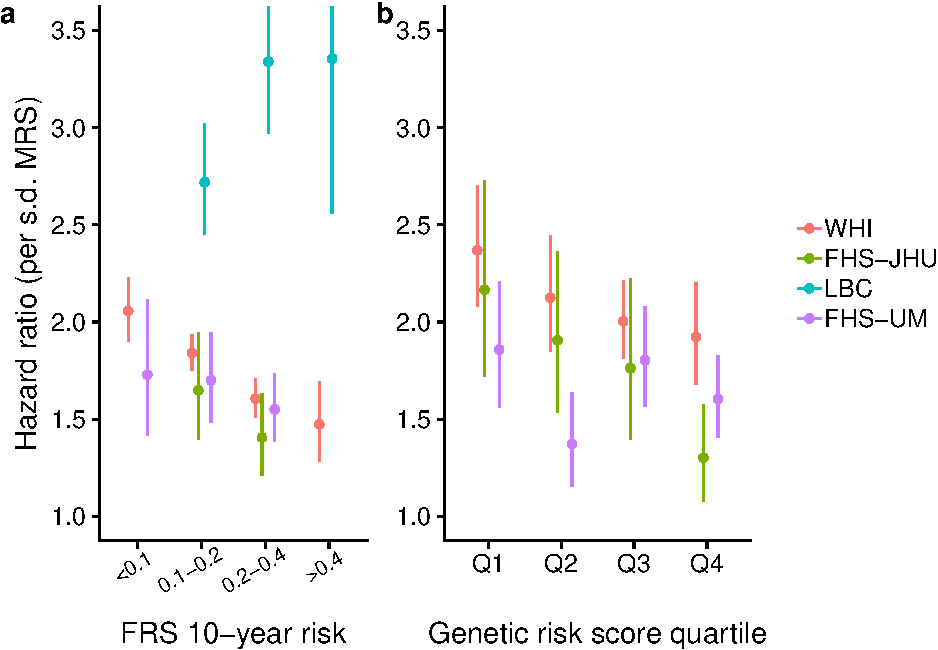
\includegraphics{../doc/mrs_models/figures/interactions-1.pdf}
\caption{\label{fig:interactions}Interactions of MRS with other biomarkers of CVD risk. a) Hazard ratios for the MRS within subsets of 10-year generalized CVD risk according to the Framingham Risk Score. b) Hazard ratios for the MRS within quartiles of a genetic cardiovascular risk score (in white participants only for WHI). Hazard ratios are estimated using the final MRS, which was trained using each of these datasets. Stratum-specific Cox regressions were adjusted for age, sex, and estimated cell subtype fractions. Estimates for strata with less than 25 incident events are not shown. Error bars represent standard errors for the hazard ratio estimates (cut off above in panel (a) for ease of visualization of other points).}
\end{figure}


\end{document}
